\documentclass[a4paper]{extarticle}
\usepackage[T2A]{fontenc}
\usepackage[utf8]{inputenc}
\usepackage[english,russian]{babel}
\usepackage{minted}
\usemintedstyle{perldoc}
\usepackage[hidelinks]{hyperref}
\usepackage{graphicx}
\graphicspath{{images/}}
\usepackage[a4paper, top=20mm, left=30mm, right=10mm, bottom=20mm]{geometry} 
\usepackage{setspace}
\onehalfspacing

\begin{document}
\begin{center}
        
    \vspace{0.4cm}
    \large
    Установка и настройка tulipe/jenkins/kallithea
        
    \vspace{0.4cm}
    \textbf{Дороничев-Тедерсон Даниил, гр. ИВТ-32-БО}
       
    \vspace{0.3cm}
    \href{mailto:daniildorted@gmail.com}{daniildorted@gmail.com}
\end{center}

\section{Используемые средства}

\begin{itemize}
\item Ubuntu Linux 20.04
\item Docker v19.03.13
\item docker-compose v1.27.4
\end{itemize}

\section{Описание файла docker-compose.yml}

\begin{figure}[h!]
\begin{minted}{yaml}
version: '3.2'
services:
    jenkins:
        container_name: jenkins
        build:
            context: jenkins
            dockerfile: Dockerfile-alpine
            args:
               JENKINS_VERSION: 2.235
        ports:
           - 8080:8080
           - 50000:50000
        volumes:
           - /tmp:/var/jenkins_home/secrets/
    gitea:
        container_name: gitea
        build:
            context: gitea
        ports:
            - 222:22
            - 3000:3000
    openproject:
        container_name: openproject
        build:
            context: openproject
        ports:
            - 5432:5432
            - 8090:80
\end{minted}
\caption{структура файла docker-compose.yaml}
\label{fig:dcy}
\end{figure}

На рис. \ref{fig:dcy} можно видеть структуру файла dpcker compose. На каждый из трёх компонентов приходится свой компонент \texttt{services}. Контекстом каждого компонента по сути является отдельная директория. Для gitea и openproject используются Docker файлы представленные в master ветках репозиториев. Для jenkins в свою очередь используется модифицированный Dockerfile на основе alpine (модификация заключалась в изменении версии на более новую, а также удаление хеша  проверки целостности SHA512, так как присутствующий хэш относился к старой версии jenkins). Необходимость наличия директивы \texttt{volumes} в описании jenkins обусловлена тем, что нам необходимо получить секретный одноразовый ключ необходимый при первом запуске всей	инсталяции.
Все порты проброшены согласно стандартной документации на каждый продукт, так имеем:

\begin{itemize}
\item[--] jenkins работает на порту 8080 (web) и 50000 (jenkins agent)
\item[--] gitea работает на порту 3000 (web) и 222 (для случаев использования протокола SSH при коммитах)
\item[--] openproject работает на порту 8090 (web) и 5432 (postgresql)
\end{itemize}

\section{Скрипт резервного копирования}

\begin{figure}[H]
\begin{minted}[breaklines]{shell}
#!/usr/bin/env bash

backup_func() {
	echo "Runing backup..."
	for i in \
	 $(docker ps --filter "name=kallithea|jenkins|tulipe" | tail -n+2 | awk '{  print $1 }'); do docker export -o ${i}-ci-$(date +"%m-%d-%Y").tar ${i}; \
	done
}

backup_func;

\end{minted}
\caption{Скрипт резервного копирования}
\label{fig:backup}
\end{figure}

Скрипт представлен на риc.\ref{fig:backup}. По сути данный  скрипт производит фильтрацию запущенных контейнеров по имени, и экспортирует запущенные экземпляры в tar архивы с датой и временем. Далее архивы можно загрузить вновь используя команду 
\texttt{docker load -i <archive\_name.tar>}

\section{Демонстрация установки}

\begin{figure}[H]
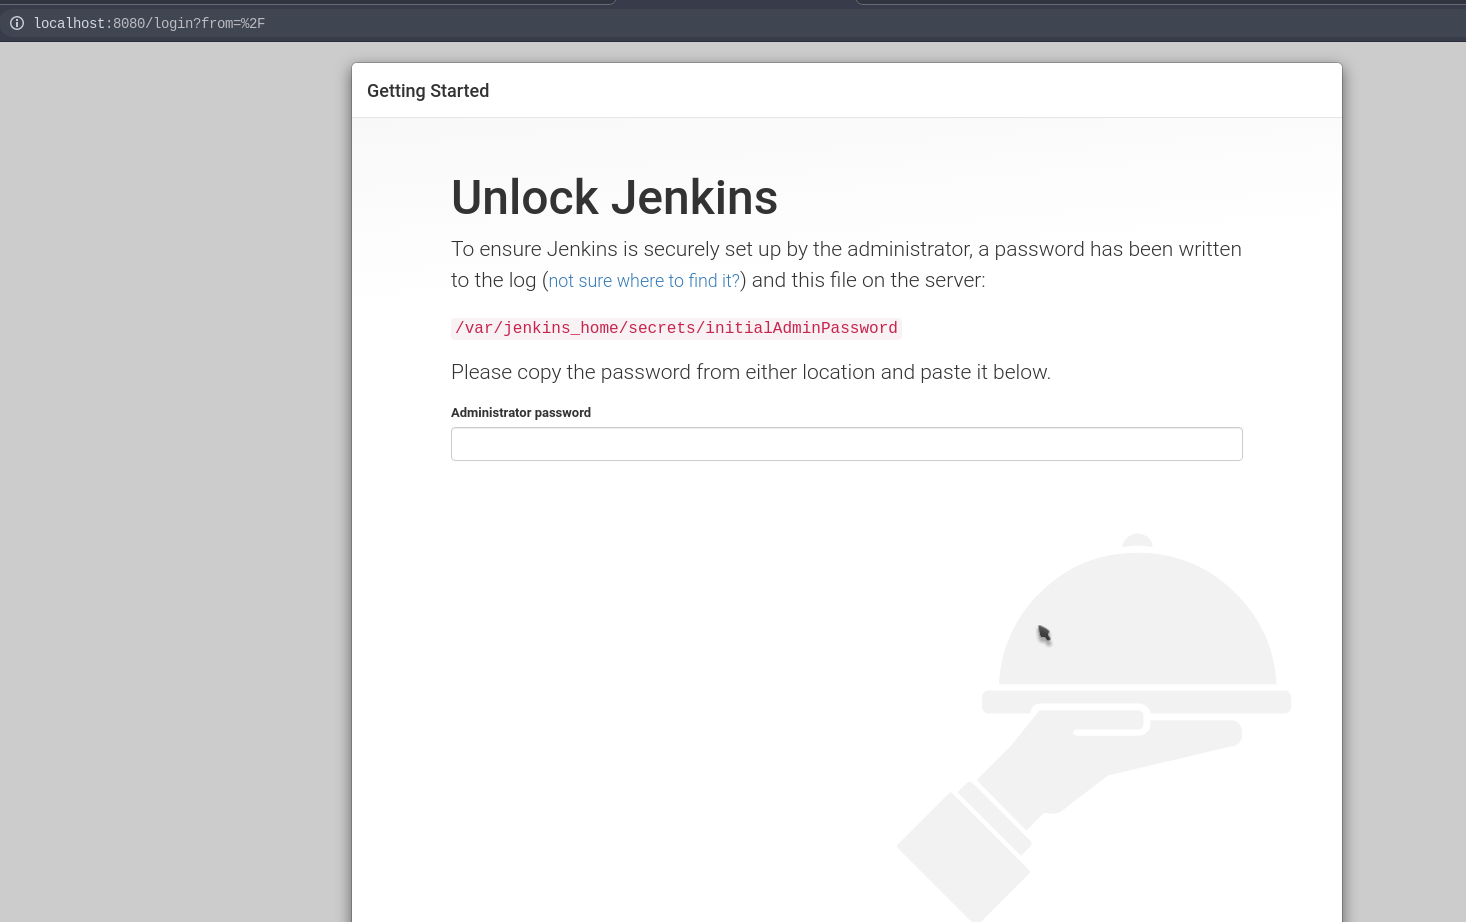
\includegraphics[width=\textwidth,height=\textheight,keepaspectratio]{jenkins_setup.png}
\caption{Начальный экран jenkins, с запросом уникального ключа}
\end{figure}

\begin{figure}[H]
\includegraphics[width=\textwidth,height=\textheight,keepaspectratio]{gitea_import.png}
\caption{Пример gitea с импортированным личным проектом}
\end{figure}

\begin{figure}[H]
\includegraphics[width=\textwidth,height=\textheight,keepaspectratio]{jenkins_git.png}
\caption{Пример настройки интеграции gitea и плагина jenkins git}
\label{fig:git}
\end{figure}

Для рис. \ref{fig:git} Стоит сделать уточнительное пояснение. Для интеграции необходимо указать полный http-адрес до репозитория. Формально инсталяция kallithea расположена по адресу \texttt{localhost:3000}. Однако данный адрес не является внутренним адресом подсети докера, для того-чтобы подключения прошло успешно необходим именно внутренний адрес. В данном случае он был выяснен путём запуска команды
\verb#docker inspect ${CONTAINER_ID} | grep IPAddr#, где \verb#${CONTAINER_ID}# --- идентификатор контейнера, в котором запущена инсталяция gitea. В качестве данных  для авторизации используются данные пользователя gitea.

\begin{figure}[H]
\includegraphics[width=\textwidth,height=\textheight,keepaspectratio]{shell.png}
\caption{Пример проверочной команды для выполнения по коммиту в репозиторий}
\end{figure}

\begin{figure}[H]
\includegraphics[width=\textwidth,height=\textheight,keepaspectratio]{suc_build.png}
\caption{Пример успешной сборки проекта с помощью интеграции}
\end{figure}

\begin{figure}[H]
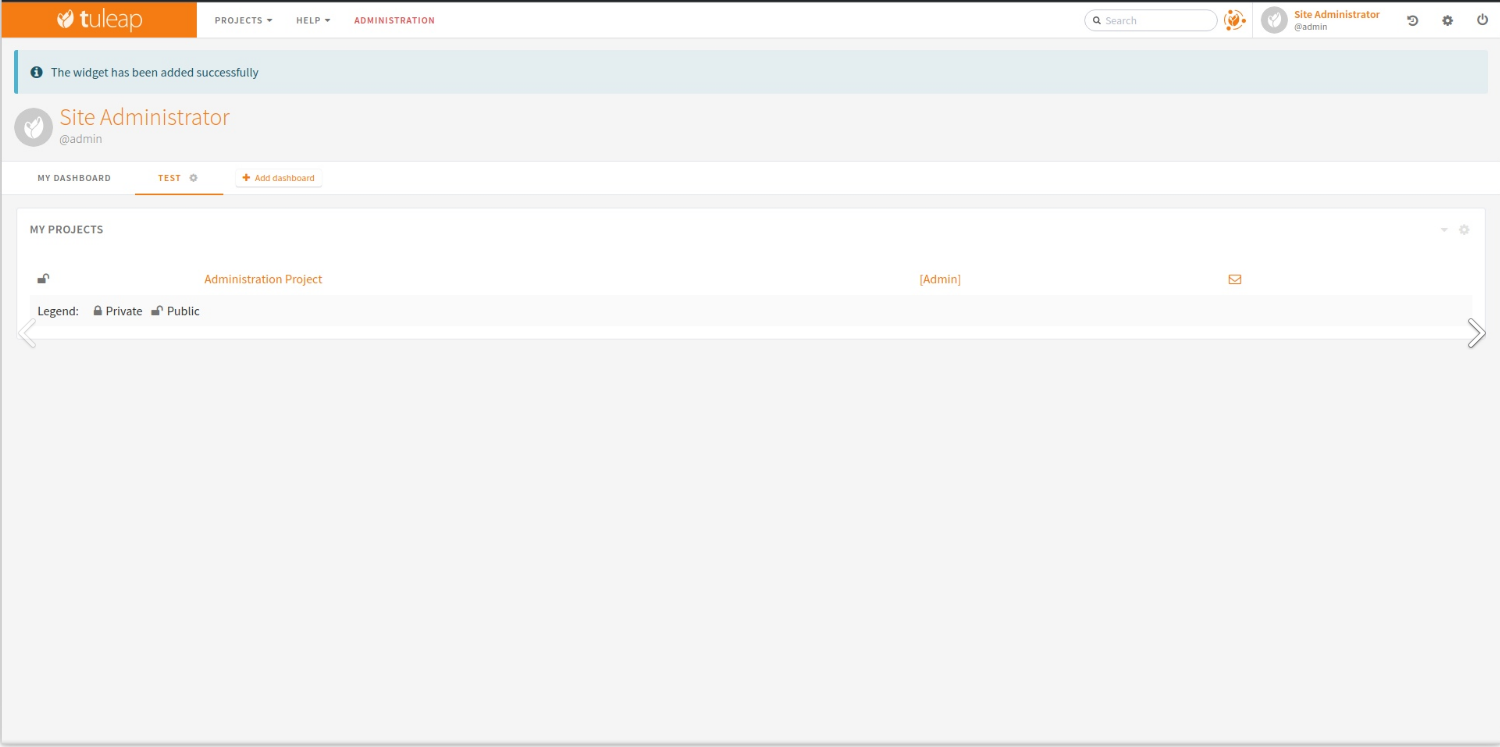
\includegraphics[width=\textwidth,height=\textheight,keepaspectratio]{tulipe.png}
\caption{Пример создания тикета в tulipe}
\end{figure}

К сожаление, согласно документации, (а также  форумам поддержки всех трёх проектов), не существует интеграции kallithea с tulipe или tulipe с jenkins.

\end{document}